
\label{subsec:ANN:NARX}

The nonlinear autoregressive network with exogenous inputs (NARX) is a
recurrent dynamic network; \ie, it has feedback connections.  Based on
the linear ARX models, NARX ones have been demonstrated suitable for
modeling nonlinear systems and specially time series.

The simplest NARX network consists on a feedforward neural network
with a first TDL at the input plus a delayed connection from the
output to the input layer (a second TDL).
\figref{narx} shows a schematic version of this NARX network.

\begin{figure}[!ht]
\centering
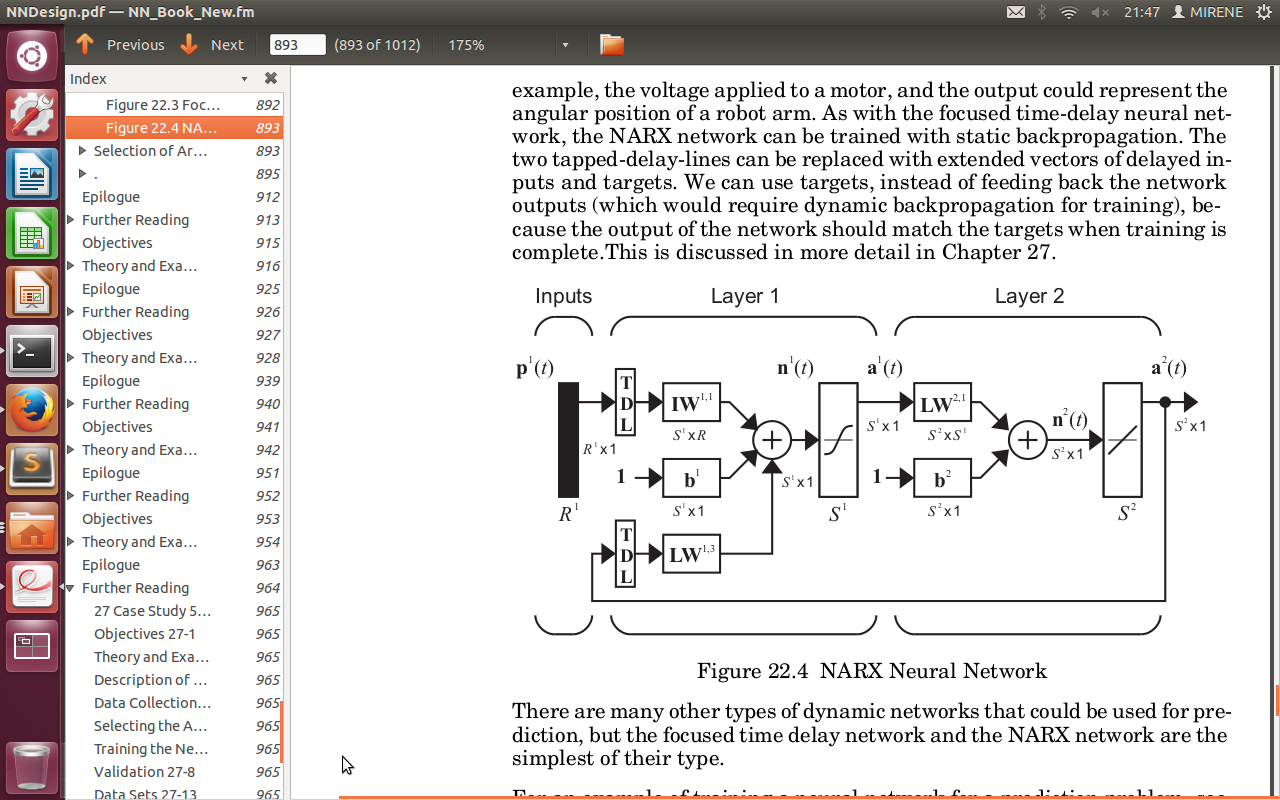
\includegraphics[width=\textwidth]{images/narx.png}
\caption{NARX network}
\label{fig:narx}
\end{figure}

The defining general equation of an one-step-ahead ARX model is
% \begin{equation}
% \begin{split}
% y(t) =f(y(t-1),y(t-2),...,y(t-n_{y}), \\
% u(t-n_{k}),u(t-(n_{k}+1)),...,u(t-(n_{k}+n_{u})))
% \end{split}
% \end{equation}
\begin{equation}
\hat{y}(t) =f(\hat{y}(t-1),\hat{y}(t-2),...,\hat{y}(t-d_{y}), u(t-1),u(t-2),...,u(t-d_{u}))
\label{eq:narxequation}
\end{equation}
where the value of the dependent output signal $\hat{y}(t)$ is
regressed on the $d_{y}\geq1$ previous values of the same output
signal and $d_{u}\geq0$ previous values of the independent exogenous
input signal $u(t)$ \cite{lin1996learning}.  The unique dissimilarity
between ARX and NARX models lies in the linearity of the function $f$.
Thus, in the NARX neural network of \figref{narx}, $f$ is a
combination of the non-linear activation functions $\mathbf{f}^1$ and
$\mathbf{f}^2$.

%The prediction horizon $n_{k}$ is defined as the shift among corresponding input and output values so that current input is used for predicting the output in $n_{k}$ time steps in the future.

In what concerns training a NARX network the
named \emph{Backpropagation Through Time} version of the
backpropagation algorithm can be used (read \subsecref{bptt}). The
process can be carried out in one out of the two modes shown
in \figref{narxtrainingarch} \cite{menezes2008long}:
\begin{itemize}
	\item Parallel architecture, where the output $\hat{y}(t)$ is
	fed back to the input of the feedforward neural network as
	part of the standard NARX architecture.  

        \item Series-parallel architecture, in which the true output
	$y(t)$ -well-known target output- is used instead of feeding
	back the estimated output $\hat{y}(t)$.
\end{itemize}

Idially, NARX networks are trained with the series-parallel architecture and tested with the only parallel one.

\begin{figure}[!ht]
\centering
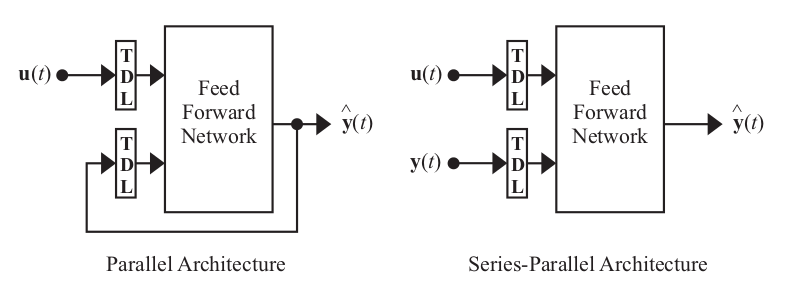
\includegraphics[width=\textwidth]{images/narxTrainingArchitectures.png}
\caption{NARX network training architectures}
\label{fig:narxtrainingarch}
\end{figure}



